We can now focus on the single nodes of our systems: \textbf{servers}.
\begin{figure}[H]
    \centering
    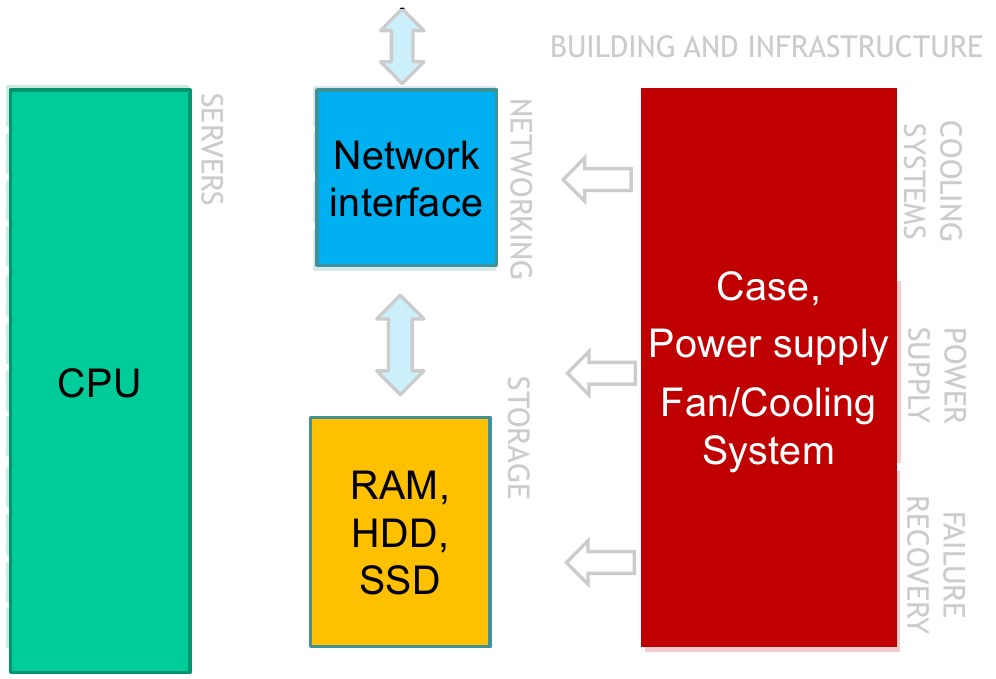
\includegraphics[width=0.8\textwidth]{Images/10ServerArchitecture.png}
    \caption{General Server Architecture}
\end{figure}
Servers can be considered as the basic building block of our DC, there exists
several configurations and combinations of different types of servers (for 
bigger and smaller businesses) but all different assets are accomunated by the
basic needs of a server in order to be called like that:
\begin{itemize}
    \item \textbf{The Motherboard} - the central hub of the single server unit, 
    connecting all components altoghether 
    \item \textbf{Chipsets} - the main computational components, such as CPU,
    RAM, GPUs and main memory components.
\end{itemize}
Different types of servers are also to be considered:
\begin{itemize}
    \item \textbf{Tower} - optimal for scalable solutions and easy cooling, but
    used only in businesses that require basic level of performance. Also 
    consumes a lot of space and cable management is a nightmare.
    \item \textbf{Rack} - optimal for space usage and with racks (the shelves)
    an even better unified and interconnected system: unified because all is
    compared to units (1U = 44.45mm of height) to have the best rack 
    organization. Their density often implies that they require more power to 
    cool off and most importantly a certain difficulty in maintaining and 
    replacing faulty ones.
    \item \textbf{Blade} - the latest type of servers, that function as a 
    hybrid rack system. More compact, small, versatile and modular, meet the 
    IEEE U standard for racks: they increase "packingness" at the cost of 
    having a higher initial cost, possible vendor lock-in (no cables, only 
    specific enclosures that are made by specific manufacturers) and a big
    need of cooling.

\end{itemize}
\begin{figure}[H]
    \centering
    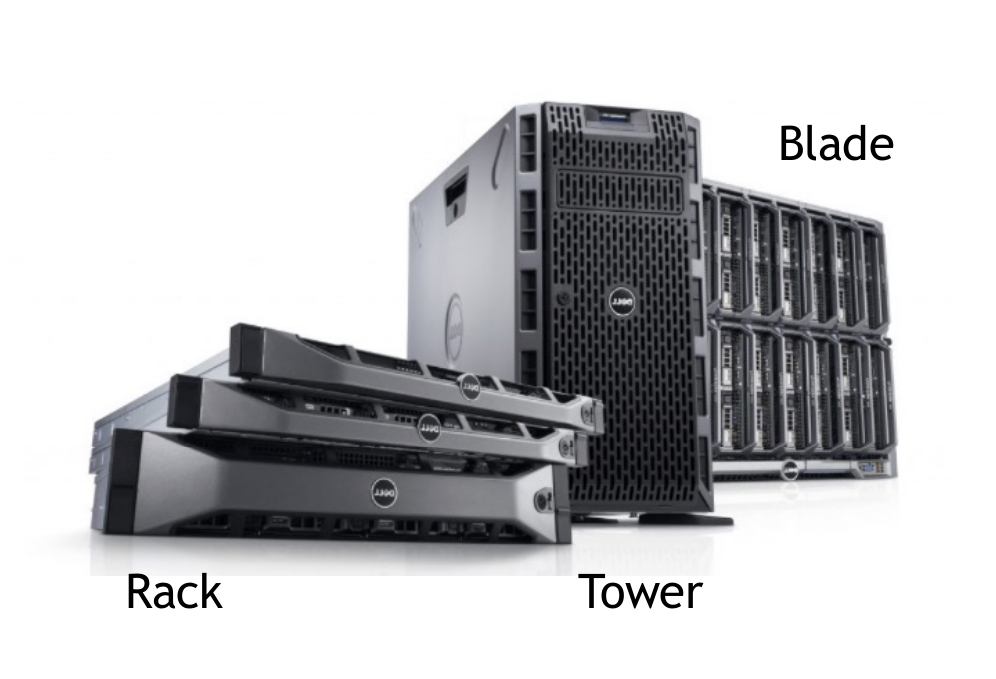
\includegraphics[width=0.8\textwidth]{Images/11ServerTypes.png}
    \caption{All Server Types}
\end{figure}

\subsection{Accelerators and ML Era}
The need of more complex model inside the industry led to new hardware to try
to "accelerate" the all neural models and their computational load: let's 
define some basis of AI and Machine Learning to understand how those 
accelerators work
\begin{key}{Artificial Neural Network}
    An ANN is a human inspired computational model where interconnected nodes 
    (neurons) are organized in layers and are instructed to process and analyze
    data.
\end{key}
Single neurons are connected with weighted connections, that are strenghtened 
or weakened through training: initially, those are randomly initialized. That's 
how, with the advent of more powerful CPUs, Deep Learning started to take place.
Since 2013, AI training compute requirements have doubled every 3.5 months, 
that's why accelerators were needed to speed up the training process of a model.
The first solution that came to mind is the usage of GPUs, which have high 
compute density and are built for parallel operations with high throughput: 
more threads to work with and with deep pipelines with multiple stages.
\begin{figure}[H]
    \centering
    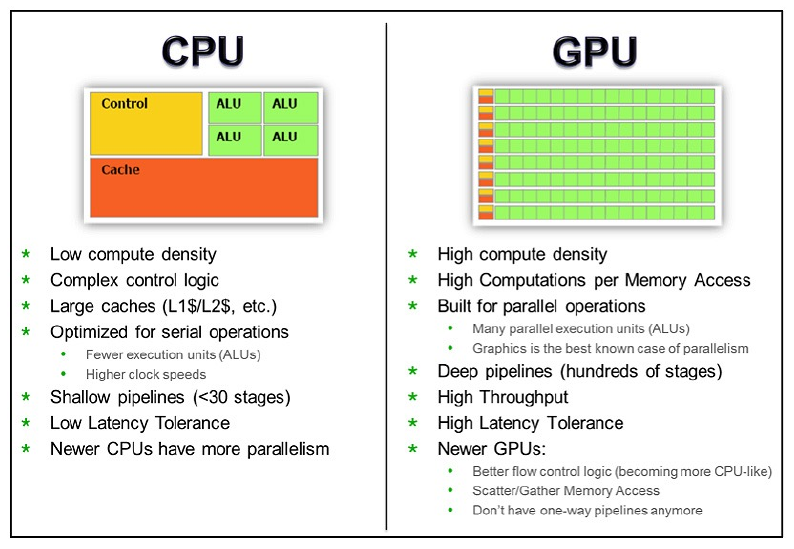
\includegraphics[width=0.9\textwidth]{Images/12GPUs.png}
    \caption{CPUs vs GPUs}
\end{figure}
Appropriate languages are to be used to program on these GPUs, such as CUDA.
Once a network of GPUs is established, it is possible to determine the speed of
the training by watching the slower GPU of the batch: every GPU does its 
calculations, then follow a back-propagation algorithm to update the weights on
the connections and finally all informations are updated between all nodes.
\textbf{It is crucial that the whole system is well connected.}
Finally, the system is structured with this layout (as example): GPUs are 
connected with high-bandwidth connectors (such as NVlink) to minimize latency, 
a CPU hosts is connected to the accelerator with a PCI-express.
\subsection{Tensor Processing Units}
Since GPUs are still general purpose devices, Google decided to implement a
device specialized in ML training: by having next to zero overhead efficiency
is maximized.

Go on until page 45
